\documentclass[11pt]{article}
\usepackage{geometry}
\usepackage{fullpage}
\usepackage{graphicx}
\usepackage{tabularx}
\usepackage{url}
\newcolumntype{T}{>{\centering\arraybackslash}m{0.20\textwidth}}
\newcolumntype{L}{>{\centering\arraybackslash}m{0.74\textwidth}}
\geometry{a4paper}
\setlength\parindent{0pt}
\title{Deliverable 6}
\author{
    Gordon Reid: 1002536R\\
    Ryan Wells: 1002253W\\
    Kristopher Stewart: 1007175S\\
    David Selkirk: 1003646S\\
    James Gallagher: 0800899G\\
}
\date{\today}

\begin{document}

\maketitle

\newpage

\tableofcontents

\newpage

\section{Introduction}

\subsection{Identification}

This is the design document and test plan for the internship management system
being developed by Team W for the Professional Software Engineering 3 course.
The internship management system is for Software Engineering (SE) and Electronic
and Software Engineering (ESE) students, studying in the school of Computing
Science.

\subsection{Related Documentation}

PSD3 Group Exercise Description:

\url{fims.moodle.gla.ac.uk/file.php/128/coursework/psd3-ge-2.pdf}

\subsection{Purpose and Description Of Document}

This document serves as the design document containing the overall system
architecture diagram with associated state charts. Each component in the
system architecture also has its own class diagrams and API specifications
specified.

\subsection{Document Status and Schedule}

This document is the draft version of the deliverable and is subject to major
change.

\newpage

\section{System Architecture}

\subsection{Diagram}

\begin{centering}
  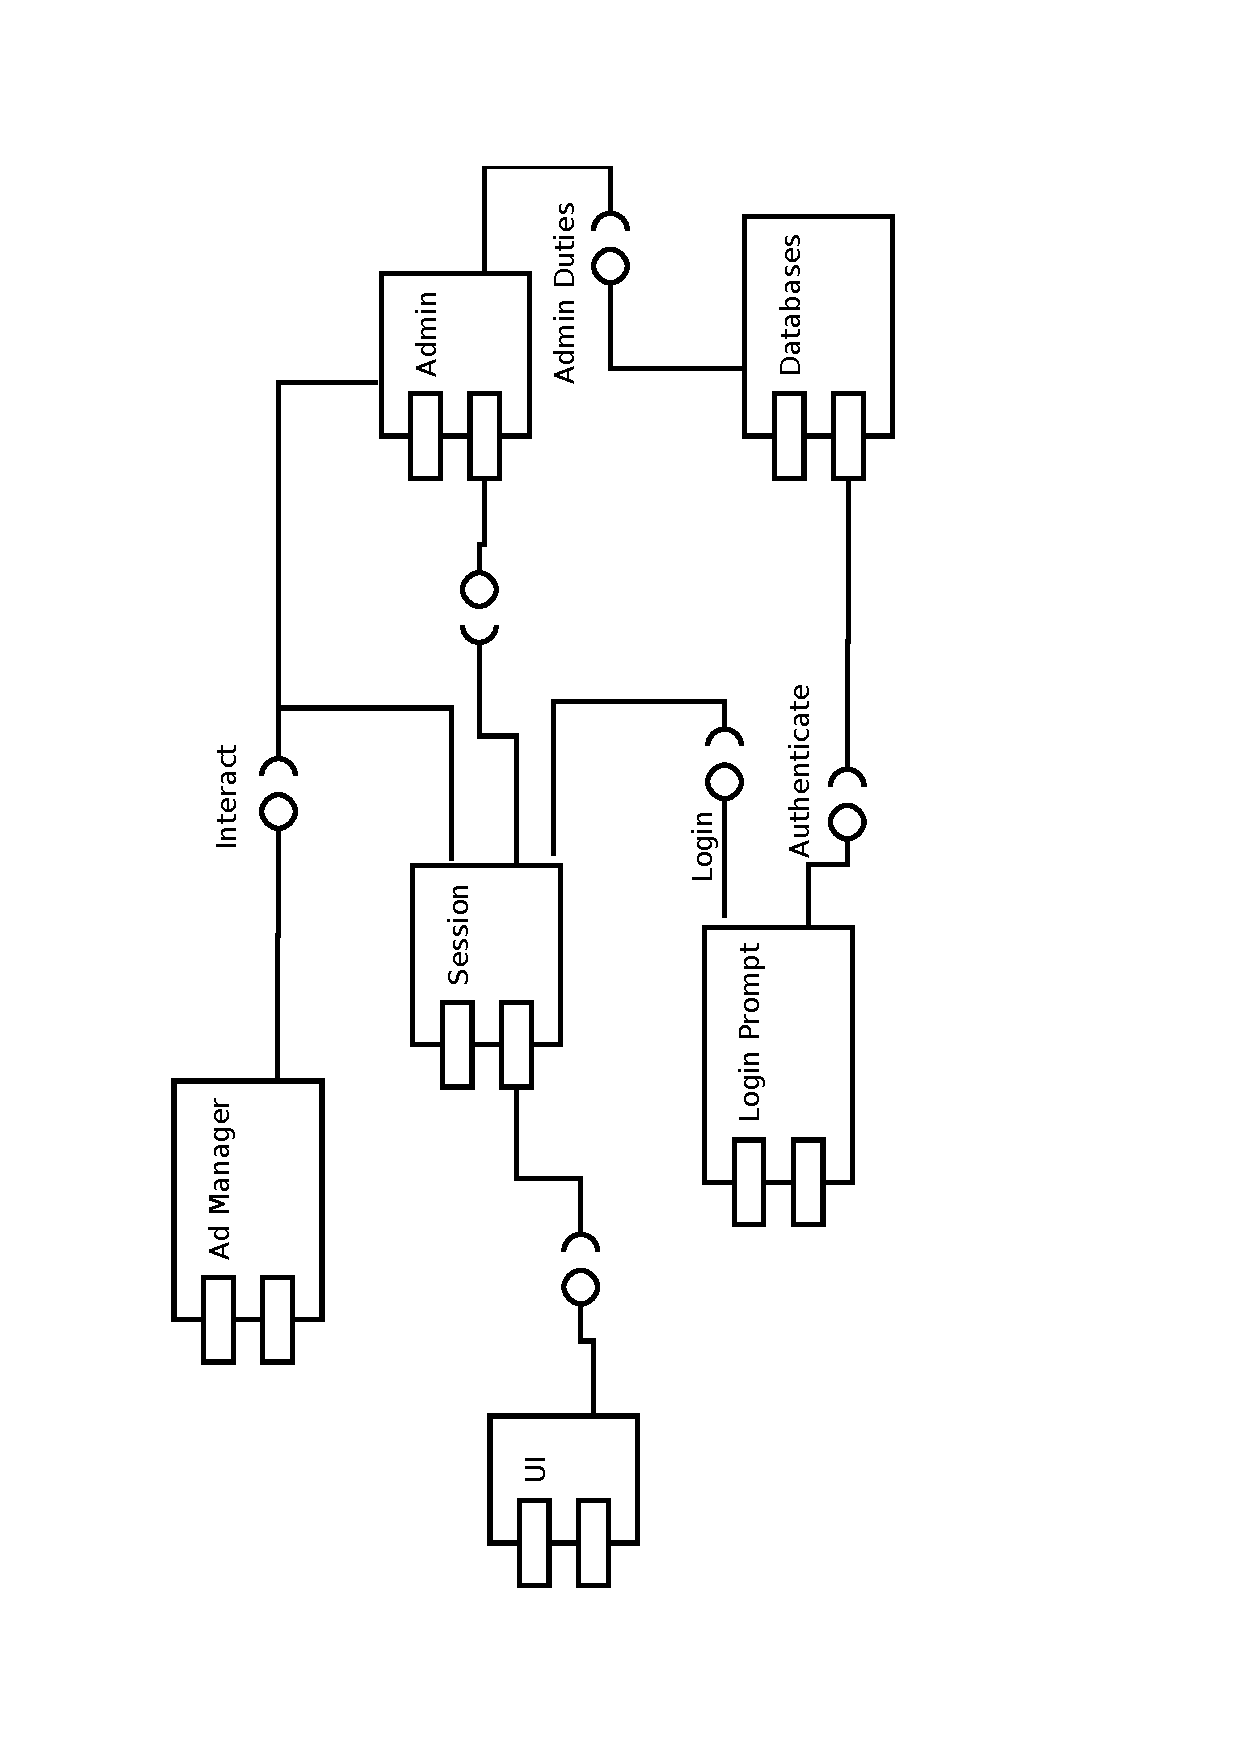
\includegraphics[width=0.7\textwidth,angle=270]{PSDDiagram.pdf}
\end{centering}

\subsection{Rationale}

We decided upon this system architecture as any component of the system should 
have the properties of being interchangeable with another substitutable 
component (substitutable defined as being having the same API). For this reason, 
we grouped relatable functionalities together and made them into a component. 
The ``Ad Manager'' and the ``Databases'' components could be combined together 
into one large ``Database'' component, but we did not want to create a coupling 
between these components - the ``Ad Manager'' may well have a database inside 
it, but the information inside this database is managed in a different way from 
the other data in the system such as users and companies.

All other components are defined by the primary reason that any component in the 
system can be replaced with no effect to the overall working of the system.

\newpage

\section{State Charts}

\subsection{Advertisement}

\subsubsection{Diagram}

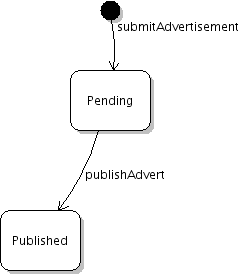
\includegraphics{advertState.png}

\subsubsection{Rationale}

The form of the state chart was decided based on the simplistic nature of an 
advertisements status. All adverts start off life as pending, after a company
has made the initial submission. They can be revised at any time prior to either
being declined by the course coordinator, where they are removed from the system
(and feedback sent to the company) or published for viewing.

An addition (which requires clarification) is the `Position Filled' state and
associated end state. This is asked in the questions section at the end of the
document. As such, that part of the diagram is under review pending further
information.

\subsection{Student}

\subsubsection{Diagram}

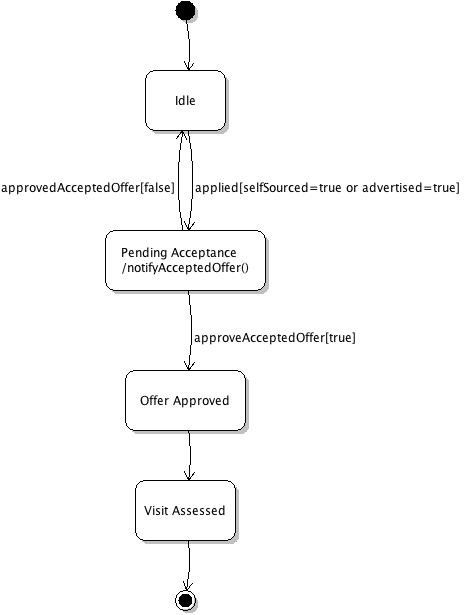
\includegraphics[width=\textwidth]{studentState.png}

\subsubsection{Rationale}

We decided to create a state chart for a Student's flow throught the
system as to clarify the functionality of the system with relation to
the student, and also for a base reason of a student having a
different state at multiple points in the system. There are various
paths that a student can take through this system and ultimately
result in the same final state, this is modelling the best case
scenario for a student where a student will eventually end up with an
approvable final placement, which we have interpreted as being one of
the main functionalities of the system. 

A student contunally changes state between ``Idle'' and ``Pending
Acceptance'' (through either ``Applied for Position'' or ``Found Self
Sourced Role'') potentially multiple times until a suitable position
has been found and only then they will progress on to ``Offer
Approved''. A Student will then be stagnant until a visit has been
undertaken and then the student will terminate. A visit is outside the
control of the Student, so it will stay in this state until changed by
an outside element.

\newpage

\section{Class Diagrams and API Specifications}

\subsection{Advert Manager}

\subsubsection{Class Diagram}

\subsubsection{API Specification}

\subsection{Session}

\subsubsection{Class Diagram}

\subsubsection{API Specification}

None. Possibly extend this to include Main/run?

\subsection{User Interface}

\subsubsection{Class Diagram}

\subsubsection{API Specification}

\textbf{Full name:} public abstract interface InternManCommanLineUI\\

\textbf{Package:} uk.ac.glasgow.internman.ui

This is the interface for the ui.

\begin{itemize}

\item{\textbf{public void run()}

Runs the UI.

\textbf{Preconditions:} 

\textbf{Invariants:}

\textbf{Postconditions:} UI is displayed.}

\end{itemize}

\subsection{Admin}

\subsubsection{Class Diagram}

\subsubsection{API Specification}

\textbf{Full name:} public abstract interface Admin\\

\textbf{Package:} uk.ac.glasgow.internman.admin

This is the interface for the administration part of the database, accessible by
only the course coordinator.
This assumes that the user using this interface has Course Coordinator
rights.

\begin{itemize}

\item{\textbf{public void approveAdvertisement(Advertisement advertisement)}

Approves an advertisement.

\textbf{Preconditions:} Advertisement must be in advertisement database.

\textbf{Invariants:}

\textbf{Postconditions:} Advertisement is now approved.}

\item{\textbf{public boolean addCompany(String name, String email, String
    password)} 

Interface to add a company to the database, functionality is delegated to the
database component.
Error checking is done inside this function, but not whether or not a company
currently exists inside the companies database.

\textbf{Preconditions:} 

\textbf{Invariants:}

\textbf{Postconditions:} The return value of the delegated function indicates
the success of this function.}

\item{\textbf{public void approveAcceptedOffer(String matriculation)}

Approves the offer most recently accepted by the student with this matriculation
id. 
\textbf{Preconditions:} Student with this matriculation must have a successful
application and must have notified the Course Coordinator of their success.

\textbf{Invariants:} Student must not accept another successful application
during this review process.

\textbf{Postconditions:} Students status is changed to a success status.}

\item{\textbf{public void assignAcademicVisitor(String matriculation, String
    visitorName)}
Sends email to student, visitor and employer manager to let them know about
assignment. 

\textbf{Preconditions: An academic visit cannot be currently assigned.}

\textbf{Invariants:} 

\textbf{Postconditions:} }

\end{itemize}
\subsection{Login Prompt}

\subsubsection{Class Diagram}

\subsubsection{API Specification}

\subsection{Database}

\subsubsection{Class Diagram}

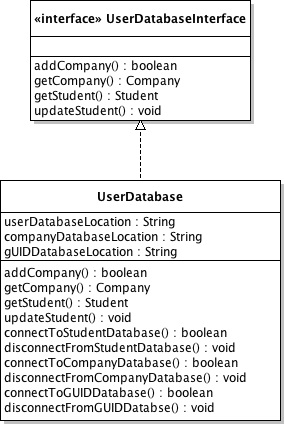
\includegraphics{databaseClassDiagram.png}

\subsubsection{API Specification}

\textbf{Full name:} public abstract interface UserDatabase\\

\textbf{Package:} uk.ac.glasgow.internman.users

This is the interface for the user database. This database will hold information
on students, companies, and the course coordinator. For University students and
staff members, the database will access the MyCampus GUID system for login. For
companies, a separate store for their user information will be used.\\

\textbf{Methods}

\begin{itemize}

\item{\textbf{public boolean addCompany(String name, String email, String 
password)}

Add information about a company to the database.

\textbf{Preconditions:} Database must not already contain details of the 
company.

\textbf{Invariants:}

\textbf{Postconditions:} Database now contains information about a company 
including their login password.}

\item{\textbf{public Company getCompany(String name)}

Gets information about the company with the given name.

\textbf{Preconditions:}

\textbf{Invariants:}

\textbf{Postconditions:} If a valid name is given, the object associated with
the company is returned, otherwise null is returned.}

\item{\textbf{public Student getStudent(String guid)}

Gets information about the student with the given GUID from MyCampus and the
application's user specific information database (such as internship progress).

\textbf{Preconditions:}

\textbf{Invariants:}

\textbf{Postconditions:} If a valid GUID is given, the object associated with
the student is returned, otherwise null is returned. If this is the first time
a student has been asked for, a record will be added to the user specific
information database.}

\item{\textbf{public void updateStudent(Student student)}

Updates the user specific data for the supplied student. For example, when a
student obtains an internship, or has had their internship assessed.

\textbf{Preconditions:} Student must be a valid Computing Science student and
is known to the application's user database.

\textbf{Invariants:}

\textbf{Postconditions:} Student's user specific information is up to date.}

\end{itemize}

\newpage

\section{Acceptance Test Plan}

\begin{tabularx}{\textwidth}{|T|L|}
\hline
Identifier & UtilityTCLogin1\\
\hline
Use Case & Login\\
\hline
Setup &\\
\hline
Interface & uk/ac/glasgow/internman\\
\hline
Includes &\\
\hline
Procedure & JUnit Test Case: uk/ac/glasgow/internman/tests/accept/LoginStudent\\
\hline
Inputs & String username: "9876543A", String password: "LetMeIn"\\
\hline
Outcome & Student with GUID 9876543A is set as the current user of the system.\\
\hline
\end{tabularx}

\begin{tabularx}{\textwidth}{|T|L|}
\hline
Identifier & UtilityTCLogin2\\
\hline
Use Case & Login\\
\hline
Setup &\\
\hline
Interface & uk/ac/glasgow/internman\\
\hline
Includes &\\
\hline
Procedure & JUnit Test Case: uk/ac/glasgow/internman/tests/accept/LoginCompany\\
\hline
Inputs & String username: "TestCompany", String password: "LetMeIn"\\
\hline
Outcome & Company name "TestCompany" is set as the current user of the system.\\
\hline
\end{tabularx}

\begin{tabularx}{\textwidth}{|T|L|}
\hline
Identifier &\\
\hline
Use Case &\\
\hline
Setup &\\
\hline
Interface &\\
\hline
Includes &\\
\hline
Procedure &\\
\hline
Inputs &\\
\hline
Outcome &\\
\hline
\end{tabularx}

\newpage

\section{Requirements Specification Questions}

\begin{itemize}

\item{Employers are required to register however during the registration process
only the company name and email is supplied (registerNewEmployer()). However,
users are required to supply their username and password to login. Based on the
assumption that the employer/company name is the username, what would the
password initially be set to?}

\item{How does the course coordinator decline an offer a student has received?}

\item{When and how does an approved/published advertisement disappear from the 
set of available advertisements?}

\end{itemize}

\end{document}
